\section{Modulation techniques}
\label{sec:sisoModulation}
\graphicspath{{_SISO/Figures/}}

The optical carriers span the electromagnetic spectrum within 380 THz -- 780 THz range. Lack of adequate electronics for passband transmission or reception at such high frequency ranges makes it impractical to implement coherent signaling schemes. However, it is possible to vary the intensity of such spectrum at the transmitter and detect it directly by optical flux to electrical signal conversion at the receiver. Thus, modulation techniques are implemented in conjunction with IM/DD to transfer information using the optical spectrum. A number of different modulation techniques have been studied for RF wireless communications. Some of those have been adapted for OWC due to the unique constraints of the optical channel. This section provides a summary of the more popular SISO modulation techniques.

\subsection{On-off keying}
\label{subsec:sisoModulationOOK}
\begin{figure}[!b]
	\centering
		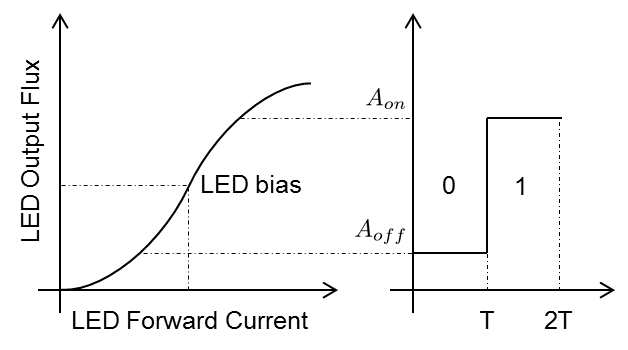
\includegraphics[trim={0in 0in 0in 0in}, clip=false, width=4in]{Signal_OOK.png}
		\caption{Optical OOK signals}
		\label{fig:sisoSigOOK}
\end{figure}
As the name suggests, OOK transmits information in the form of presence (on) or absence (off) of light. It is typically implemented under the NRZ model. To transmit bit `0', the transmitter drives all LEDs at a low intensity level and to transmit bit `1', it drives them all to a high intensity level. The on and off intensity levels can be set to achieve a desired average illumination level. \figurename{ \ref{fig:sisoSigOOK}} illustrates the OOK signal waveforms. $A_{off}$ is the low intensity radiant flux and $A_{on}$ is the high intensity radiant flux emitted by the LEDs at the off and on levels. If $p$ is the probability of transmitting bit `1', the average transmitted flux given by $A_{avg} = (1-p)A_{off} + pA_{on}$ is used to provide illumination whereas flux $A_{com} = p(A_{on}-A_{off})$ is used for communication. OOK-NRZ has a spectral efficiency of 2 bits/Hz. References \cite{kom04a,vuc09b} have demonstrated feasibility of OWC in indoor spaces while providing illumination using OOK.


\subsection{Pulse amplitude modulation}
\label{subsec:sisoModulationPAM}
\begin{figure}[!t]
	\centering
		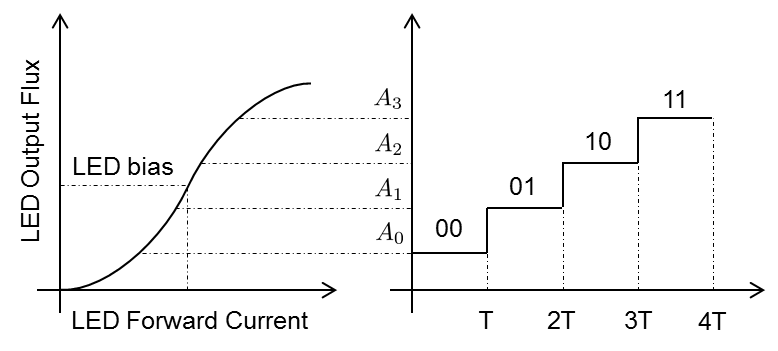
\includegraphics[trim={0in 0in 0in 0in}, clip=false, width=5in]{Signal_4PAM.png}
		\caption[Optical PAM signals]{Optical 4-PAM signals}
		\label{fig:sisoSig4PAM}
\end{figure}
$M$-ary PAM can transfer information by varying the amplitude of each transmitted pulse. $m$=log$^{ }_{2}(M)$ bits to transmit are mapped to one out of $M$ possible pulse amplitudes. To transmit $m$ bits, the transmitter then drives all LEDs to emit radiant flux corresponding to the mapped amplitude. Let $A_{lo}$ be the lowest pulse amplitude and $A_{hi}$ be the highest pulse amplitude, then the $M$ different amplitude levels are given by $A_{i} = A_{lo} + i\times(A_{hi}-A_{lo})(M-1); 0\leq i<M$. For equi-probable bits, flux given by $A_{avg} = (A_{lo} + A_{hi})/2$ is used to provide illumination whereas flux $A_{com} = (A_{hi}-A_{lo})/2$ is used for communication. \figurename{ \ref{fig:sisoSig4PAM}} illustrates the $4$-PAM signal waveforms. References \cite{gru08b} have demonstrated $M$-ary PAM for OWC in indoor spaces while providing illumination.


\subsection{Pulse position modulation}
\label{subsec:sisoModulationPPM}
$M$-ary PPM can transfer information by varying the temporal offset (position) for the low-high edge of each transmitted pulse. The amplitude and duty cycle of each pulse is kept constant. $m$=log$^{ }_{2}(M)$ bits to transmit are mapped to one out of $M$ possible pulse offsets. 
\begin{figure}[!t]
	\centering
		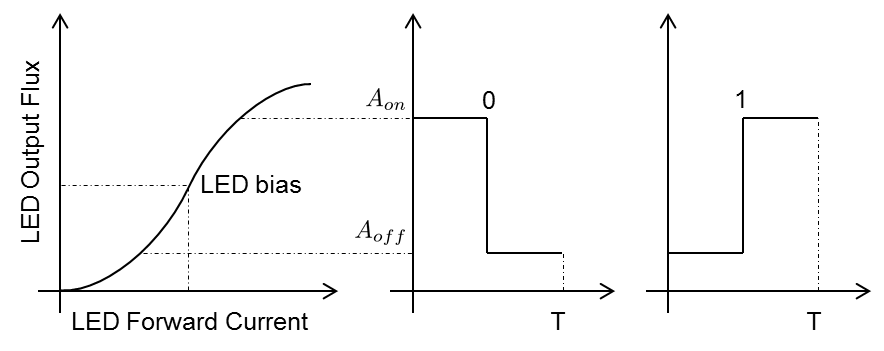
\includegraphics[trim={0in 0in 0in 0in}, clip=false, width=5.5in]{Signal_2PPM.png}
		\caption[Optical PPM signals]{Optical 2-PPM signals with 50$\%$ duty cycle.}
		\label{fig:sisoSig2PPM}
\end{figure}
To transmit $m$ bits, the transmitter drives all LEDs to emit a constant flux for a constant pulse on-time starting at a corresponding mapped temporal offset. Let $A_{off}$ be the low intensity radiant flux emitted during the off time of each pulse period and $A_{on}$ be the high intensity radiant flux emitted by the LEDs during the on time of each pulse period and let $d$ be the pulse duty cycle. Then irrespective of the distribution on the information bits, flux given by $A_{avg} = (1-d)A_{off} + dA_{on}$ is used to provide illumination whereas flux $A_{com} = d(A_{on}-A_{off})$ is used for communication. \figurename{ \ref{fig:sisoSig2PPM}} illustrates $2$-PPM signal waveforms. References \cite{bai10a} have demonstrated using PPM for illumination and communication. VPPM, a variation on PPM, has been proposed in IEEE 802.15.7  as a means to achieve dimming along with data communications. In $M$-ary VPPM, the information to transmit is still mapped to one out of $M$ possible pulse off-on edge start offsets. However, the duty cycle of each pulse can be varied to control the average amount of flux emitted and thus illumination levels. Reference \cite{raj12a} outlines using VPPM for illumination and communication.

\subsection{Optical orthogonal frequency division multiplexing}
\label{subsec:sisoModulationOOFDM}
OFDM is a spectrally efficient modulation technique and has been widely adopted for RF wireless communications. In OFDM, parallel streams of information are mapped over orthogonal frequency bins. Each bin is called a sub-carrier. Usually an $M$-ary QAM modulation is used to map information over each sub-carrier. An IFFT operation multiplexes the parallel streams to generate a time domain OFDM symbol to transmit. To mitigate interference due to multi-path, usually a CP is appended to the symbol before transmitting it. At the receiver, after removing the CP, an FFT operation demultiplexes the OFDM symbol to recover the parallel sub--carriers. Each sub-carrier is then demodulated to recover the information. OFDM has been successfully adapted and widely used for spectrally efficient OWC as summarized in reference \cite{arm09a}. For OWC, the time domain OFDM symbol is constrained to be real valued and unipolar. Ensuring Hermetian symmetry during symbol mapping over the orthogonal frequency bins will generate a real valued time domain signal. \figurename{ \ref{fig:sisoOOFDMBD}} illustrates signaling chain for O-OFDM. 

\afterpage{%
\clearpage
\begin{landscape}% Landscape page
\begin{figure}[t]
	\centering
		
\includegraphics[trim={0in 0in 0in 0in}, clip=false, width=8in]{BlockDiagramOOFDM.png}
		\caption{Optical OFDM block diagram}
		\label{fig:sisoOOFDMBD}
\end{figure}
\end{landscape}
\clearpage% Flush page
}

Let $N_{sc}$ be the total number of sub-carriers for the O-OFDM frame. In DCO-OFDM,  the information bits are mapped to $N_{dco}^{d} = (N_{sc}/2) - 1$ number of data sub-carriers. An $M$-QAM modulator then assigns an $M$-QAM symbol corresponding the mapped bits on the data sub-carriers. The remaining sub-carriers are assigned Hermetian symmetric $M$-QAM symbols to form the frequency domain DCO-OFDM frame as shown in Eq.\eqref{eqDCOFrame}. 
\begin{equation}
	\vm{X}^{f} = [0; x_{1}^{ }; \ldots; x_{N_{dco}^{d}}^{ }; 0; x_{N_{dco}^{d}}^{*}; \ldots; x_{1}^{*}]
\label{eqDCOFrame}
\end{equation}

Taking an IFFT over frame $\vm{X}^{f}$ generates a bipolar time domain symbol $\vm{X}_{b}^{t}$. In DCO-OFDM the bipolar to unipolar conversion involves adding an offset to $\vm{X}_{b}^{t}$ such that majority of the the time domain symbol is non-negative and the symbol can then be clipped at zero. For relatively large $N_{sc}$, the signal values in the time domain are distributed normally. Thus adding an offset of at least 3.2$\times$SD ensures that less than 0.1$\%$ of signal values get clipped at zero - thus significantly reducing signal distortion due to clipping at the transmitter.

In ACO-OFDM, only the odd indexed sub-carriers carry data symbols. Hermetian symmetry is then enforced to obtain real valued time domain symbol. The information bits are mapped to $N_{aco}^{d} = (N_{sc}/4)$ number of data sub-carriers. An $M$-QAM modulator then assigns an $M$-QAM symbol corresponding the mapped bits on the data sub-carriers. The frequency domain ACO-OFDM frame construction is shown in Eq.\eqref{eqACOFrame}. 
\begin{equation}
	\vm{X}^{f} = [0; x_{1}^{ }; 0; x_{2}; \ldots; x_{N_{aco}^{d}}^{ }; 0; x_{N_{aco}^{d}}^{*}; \ldots; 0; x_{2}^{*}; 0; x_{1}^{*}]
\label{eqACOFrame}
\end{equation}

Taking an IFFT over frame $\vm{X}^{f}$ generates a bipolar time domain symbol $\vm{X}_{b}^{t}$. In ACO-OFDM bipolar to unipolar conversion is achieved by simply clipping the symbol at zero. It has been shown in reference \cite{arm06a} that this clipping introduces noise only on the non-data bearing even indexed sub-carriers. Thus by simple signal processing, an estimate of transmitted signal can be reconstructed. The $N_{aco}^{d}$ data sub-carriers are then demodulated and decoded to recover transmitted information. Implementation and performance comparisons of ACO-OFDM and DCO-OFDM is shown in reference \cite{mes11a}.
